\documentclass[conference]{IEEEtran}
\usepackage{booktabs} 
\IEEEoverridecommandlockouts
\usepackage{cite}
\usepackage{amsmath,amssymb,amsfonts}
\usepackage{graphicx}
\usepackage{stfloats}
\usepackage{placeins}
\usepackage{textcomp}
\usepackage{xcolor}
\usepackage{subcaption} 
\usepackage{romannum}
\usepackage{array}
\usepackage{dblfloatfix}
\usepackage{url}
\usepackage{float}
\def\BibTeX{{\rm B\kern-.05em{\sc i\kern-.025em b}\kern-.08em
		T\kern-.1667em\lower.7ex\hbox{E}\kern-.125emX}}

\begin{document}
	
	
	\author{
		\IEEEauthorblockN{Arpit Kumar, Arpit Bhomia, Ashish Ranjan, Saurav Gupta, and Anand M. Baswade}
		\IEEEauthorblockA{Department of Computer Science and Engineering, Indian Institute of Technology Bhilai, India \\
			Email: \{arpitk, arpitba, ashishr, sauravg, anand\}@iitbhilai.ac.in}}
	
	
	\title{TeraMove: Context-Aware Reconfiguration of THz Access Points for Resilient Pervasive Connectivity}
	
	\maketitle
	
	% Previous
	% \begin{abstract}
		% The Terahertz (THz) band promises high-speed indoor
		% connectivity for 6G, but its dependence on line-of-sight
		% makes them highly vulnerable to dynamic blockages. Traditional indoor deployments rely on static Access Points (APs) and cannot adapt when physical obstructions arise
		% or crowd patterns shift, leading to low coverage. In this
		% paper, we present TeraMove, a blockage-aware framework that
		% continuously monitors human density, detects THz link degradation from dynamic blockages, and autonomously repositions
		% the AP nodes to restore pervasive connectivity. TeraMove first
		% establishes an optimal baseline layout for AP placement using
		% a Mixed Integer Linear Programming (MILP) model over 3D
		% coordinates and beam orientations, then employs a four-tier optimization that escalates from electronic beam steering to full 3D
		% node repositioning, doing physical movement only when lighter
		% adaptations prove insufficient to provide threshold coverage.
		% Evaluations in a realistic indoor environment show that crowd-induced blockages can reduce coverage percentage to 16.6\%;
		% Our algorithm recovers it to over 95\% while requiring 65\% less
		% physical displacement than other approaches that could have been used.
		% \end{abstract}
	
	\begin{abstract}
		The Terahertz (THz) band promises high-speed indoor
		connectivity for 6G, but its dependence on line-of-sight
		makes it highly vulnerable to dynamic blockages. Traditional indoor deployments rely on static Access Points (APs) and cannot adapt when physical obstructions arise
		or crowd patterns shift, leading to low coverage. In this
		paper, we present TeraMove, a blockage-aware framework that
		uses spatial human-density context to detect THz link degradation
		from dynamic blockages and adapt the AP configuration to restore
		pervasive connectivity. We describe how this context can be obtained from 3D LiDAR depth sensing; our evaluation uses an empirical pedestrian density model.
		TeraMove first establishes an optimal baseline layout for AP placement using a Mixed Integer Linear Programming (MILP) model over 3D
		coordinates and beam orientations, then employs a four-tier optimization that escalates from electronic beam steering to full 3D
		node repositioning, performing physical movement only when lighter
		adaptations prove insufficient to provide threshold coverage.
		Evaluations in a realistic indoor environment show that crowd-induced
		blockages can reduce coverage to 16.6\%; our algorithm recovers it
		to over 95\% while requiring 84.6\% less physical displacement than
		the alternative approaches evaluated.
	\end{abstract}
	
	\begin{IEEEkeywords}
		THz, Context-Aware Adaptation, Spatio-Temporal Blockage Modeling, Adaptive Infrastructure, HPSO, Dynamic Repositioning
	\end{IEEEkeywords}
	
	% Intro 
	\section{Introduction}
	
	The emergence of 6G networks is driven by applications such as holographic communication, immersive extended reality, and digital twins that demand multi-Terabit-per-second data rates with ultra-low latency. The Terahertz (THz) band (0.1--10~THz), with far more available spectrum than sub-6~GHz and millimeter-wave (mmWave) bands, is widely regarded as an enabling physical layer for 6G. However, THz signals suffer extreme path loss and molecular absorption, requiring narrow, highly directional beams with unobstructed Line-of-Sight (LoS). In populated indoor spaces, a single human crossing the beam can cause attenuation exceeding 20~dB, potentially collapsing the link.
	
	The straightforward solution is static placement optimization, fixing transmitting nodes at predetermined positions to maximize coverage. Existing methods typically treat this as a 2D problem at a uniform ceiling height. While adequate for an empty floor plan, such deployments assume the environment remains unchanged. However, human mobility continuously changes blockage conditions, and a layout providing near-perfect coverage can degrade as crowds shift.
	
	3D LiDAR offers a reliable means to capture this changing context. Recent work has demonstrated accurate human tracking and counting indoors using 3D LiDAR \cite{b27,b29}. This spatial human-density information can characterize blockage conditions, while static over-provisioning can lead to unnecessary deployment costs.
	
	We present \textit{TeraMove}, a context-aware framework that treats transmitting node deployment as a continuous adaptation problem. It uses spatial human-density information to characterize dynamic blockage and first applies a Mixed-Integer Linear Programming (MILP) formulation to minimize the number of transmitting nodes while satisfying coverage and SINR constraints. When coverage falls below a threshold, a 4-tier HPSO framework adapts the network through beam steering, height adjustment, and, when necessary, full 3D repositioning. Tier~2 recovers most of the lost coverage, while a Hungarian algorithm minimizes physical displacement when movement is required.
	
	Although focused on THz, the framework is transmitter-agnostic and can also apply to mmWave small cells, Wi-Fi APs, and 5G base stations facing dynamic LoS blockages. We use the term ``Access Points'' (APs) throughout for generality.
	
	
	The main \textbf{contributions} of this paper are:
	\begin{itemize}
		\item A MILP formulation that jointly optimizes 3D AP placement and azimuth orientation while minimizing the number of APs required to satisfy user-level SINR coverage.
		
		\item An HPSO algorithm for dynamic repositioning that prioritizes human-density-weighted coverage while penalizing unnecessary displacement.
		
		\item A 4-tier cascading architecture that escalates from beam steering to physical repositioning only when needed, improving coverage while minimizing node displacement.
	\end{itemize}
	
	
	% \section{Introduction}
	
	% The emergence of 6G networks is driven by a new class of applications, holographic communication, immersive extended reality, and digital twins, that demand sustained multi-Terabit-per-second data rates with ultra-low latency, far exceeding what current 5G infrastructure can deliver. The Terahertz (THz) band (0.1--10~THz), with orders of magnitude more available spectrum than sub-6~GHz or millimeter-wave (mmWave) bands, is widely regarded as the enabling physical layer for this next generational leap. However, THz signals suffer extreme path loss and molecular absorption, forcing transmitters to use narrow, highly directional beams that require an unobstructed Line-of-Sight (LoS) to every user. In populated indoor spaces, this LoS dependence is inherently fragile: a single human body crossing the beam can cause attenuation exceeding 20~dB, enough to collapse the link entirely.
	
	% The straightforward solution is static placement optimization, fixing transmitting nodes at predetermined positions to maximize coverage of the people in the building. Existing methods typically treat this as a 2D problem at a uniform ceiling height. While adequate for an empty floor plan, such deployments assume the propagation environment never changes. However, dynamic blockages caused by human mobility continuously reshape the interference landscape, and a layout providing near-perfect user coverage at one moment can suffer severe degradation when a crowd clusters unexpectedly. Static over-provisioning cannot anticipate every future crowd pattern and leads to prohibitive costs.
	
	% We present \textit{TeraMove}, a context-aware framework that treats transmitting node deployment as a continuous adaptation problem rather than a one-time placement. TeraMove first uses a Mixed-Integer Linear Programming (MILP) formulation to minimize the number of deployed transmitting nodes while satisfying coverage and SINR constraints. When crowd shifts degrade user coverage below a threshold, it triggers an Adaptive Particle Swarm Optimization (HPSO) engine with a 4-tier cascading architecture: Tier~1 checks whether action is needed; Tier~2 electronically adjusts beam azimuth and beamwidth at zero physical cost; Tier~3 permits minor height changes; Tier~4, as a last resort, enables full 3D repositioning. Tier~2 alone recovers the majority of lost user coverage in most scenarios. A Hungarian algorithm-based assignment further minimizes aggregate physical displacement when movement is unavoidable.
	
	% Although focused on THz, the framework is transmitter-agnostic and applies equally to mmWave small cells, Wi-Fi access points, or 5G base stations, anywhere LoS-dependent links face dynamic blockages. We use the term ``Access Points'' (APs) throughout, noting the methodology extends naturally across deployment paradigms.
	
	% The main \textbf{contributions} of this paper are:
	% \begin{itemize}
		%     \item A MILP formulation that jointly optimizes 3D AP coordinates and azimuth orientations under a complete THz channel model, minimizing the number of nodes needed to guarantee user-level SINR coverage.
		
		%     \item An HPSO algorithm for real-time dynamic repositioning, with a composite fitness function that prioritizes human-density-weighted coverage while penalizing unnecessary physical displacement.
		
		%     \item A 4-tier cascading architecture that escalates from electronic beam steering to full spatial repositioning only when needed, significantly recovering user coverage while minimizing total physical node displacement compared to alternative approaches.
		% \end{itemize}
	
	
	\section{Related Work}
	
	The THz band (0.1--10~THz) offers very large bandwidth for 6G, but
	suffers from high path loss, molecular absorption, and severe
	line-of-sight (LoS) blockage~\cite{b5,b1,b2}. Human bodies can cause
	more than 20~dB attenuation~\cite{b6}, while pedestrian density and
	mobility strongly affect THz outage and SINR~\cite{b3,b14}. These
	characteristics make static deployments vulnerable to
	spatiotemporally varying human blockage.
	
	Existing AP placement methods primarily optimize the network before
	deployment. Baswade~\textit{et al.}~\cite{b4} formulated base-station
	placement using mixed-integer optimization, while graph clustering for efficient mmWave LoS
	coverage was proposed by Alameh~\textit{et
		al.}~\cite{b7}. Such approaches provide effective initial layouts but do
	not adapt the deployment after propagation conditions change. PSO and
	its variants have also been applied to wireless optimization,
	including 3D UAV-BS placement~\cite{b15} and mmWave massive-MIMO
	beamforming~\cite{b16}.However, these approaches mainly focus on optimizing placement or communication parameters, rather than combining electronic adaptation with physical AP reconfiguration when human blockage changes.
	Physical mobility offers another means of adapting wireless coverage as user locations vary. Wireless platforms based on UAV can adjust their position in three dimensions to improve coverage and optimize their trajectories~\cite{b15,b20}. Similarly, movable APs have been studied for indoor WLANs, where the AP locations are changed according to user distribution~\cite{b21}. Movable APs further exploit spatial channel variations by dynamically changing antenna positions
	~\cite{b22}. These approaches do not jointly consider
	indoor THz beam adaptation, vertical AP adjustment, and progressive
	full-3D repositioning based on human blockage.
	
	Dynamic adaptation also requires information about human
	movement. Vision-based learning has been used to predict impending
	mmWave/THz blockages~\cite{b25}.
	Specifically, 3D LiDAR point clouds have been extensively explored for high-resolution indoor crowd counting and geometry tracking~\cite{b27,b29}. These sensing approaches can provide the spatial
	human-density information required for blockage-aware adaptation.
	
	
	% TeraMove combines these complementary directions by using a
	% MILP-optimized 3D deployment as a static baseline and a four-tier
	% cascading HPSO for runtime adaptation. The framework progressively
	% moves from zero-displacement beam adaptation (Tier~2), through AP
	% height adjustment (Tier~3), to full 3D repositioning (Tier~4) only
	% when lighter adaptations are insufficient. The Hungarian algorithm
	% then minimizes aggregate AP displacement during physical
	% reconfiguration, enabling context-aware adaptation to dynamic human
	% blockage while limiting unnecessary infrastructure movement.
	
	
	
	
	
	
	
	% \section{Related Work}
	
	% The deployment of Terahertz (THz) communication networks depends primarily on addressing key propagation challenges, which has led to research on channel modeling and deployment methodologies. The fundamental physical characteristics of the THz channel, including free-space path loss and molecular absorption, have been extensively modeled by Akyildiz \textit{et al.} \cite{b5}. Their results show that THz waves exhibit exponential decay rates that depend on atmospheric constituents, thereby making LoS links and dense APs an absolute necessity. 
	
	% Because THz waves lack the diffraction capabilities of sub-6 GHz signals, they are highly susceptible to dynamic blockages. Research into THz channel reliability has shown that human bodies act as full blockers \cite{b6}, causing sudden signal degradation often exceeding 20 dB. Therefore, probabilistic obstruction analysis is an essential prerequisite for effective network planning.
	
	% To address these challenges, some recent research has adopted different methods of AP positioning. Methods like those of Alameh \textit{et al.} \cite{b7} involve graph clustering for optimal LoS coverage and minimum number of APs. Despite their computational efficiency, heuristic and graph-based approaches may not guarantee optimality, which is critical for critical applications and benchmark performance evaluations. Such benchmarks are usually performed in a fixed height, 2D planar deployment scenario and do not consider the vertical dimension. The application of MILP to the AP placement problem formulation has been reported for
	% lower frequencies to determine globally optimal placements.
	% However, MILP formulations for such optimization problems generally rely on static obstacle locations, 2D planar deployment scenarios, or simple path loss models. They fail to incorporate real THz channel characteristics, such as the THz molecular absorption effects, the probability of dynamic human blockages, azimuth orientation, and 3D volumetric deployment geometry within the same mathematical framework. This work fills this primary research gap by incorporating all realistic THz channel characteristics into a rigorous 3D MILP solver. Furthermore, recognizing that static deployments inherently fail under shifting pedestrian crowds, we extend beyond existing literature by introducing a dynamic, hierarchical Adaptive Particle Swarm Optimization (HPSO) framework to physically adapt AP parameters and positions in real time as human blockages evolve.
	
	
	\section{System Model and Problem Formulation}
	
	% \subsection{3D Propagation and Path Loss Model}
	The indoor environment is discretized into a 3D volumetric grid. Let $\mathcal{U}$ denote the set of target user equipment locations requiring coverage, and let $\mathcal{A}$ denote the set of candidate AP locations. Let the 3D coordinates of the user device $u$ be $(x_u, y_u, z_u)$ and the candidate AP $a$ be $(x_a, y_a, z_a)$. The volumetric Euclidean distance $d_{u,a}$ is calculated as:
	\begin{equation}
		d_{u,a} = \sqrt{(x_u - x_a)^2 + (y_u - y_a)^2 + (z_u - z_a)^2}
		\label{eq:3d_distance}
	\end{equation}
	where the user height $z_u$ is fixed to a standard level, and the optimization algorithm selects an optimal AP mounting elevation $z_a$ from a discrete set of candidate heights. 
	
	The base Free Space Loss (FSL) for a signal operating at frequency $f$ over distance $d_{u,a}$ is derived from the Friis transmission equation:
	\begin{equation}
		PL_{\text{FSL}}(d_{u,a}) = 20\log_{10}\left(\frac{4\pi f d_{u,a}}{c}\right)
	\end{equation}
	where $c$ is the speed of light in vacuum. The total deterministic (line-of-sight) path loss $PL_{\text{LoS}}(u,a)$ for THz link further incorporates molecular absorption loss and static attenuation \cite{b1}:
	\begin{equation}
		PL_{\text{LoS}}(u,a) = PL_{\text{FSL}}(d_{u,a}) + PL_{\text{ABS}}(d_{u,a}) + L_{\text{static}}
		\label{eq:total_pl}
	\end{equation}
	where $PL_{\text{FSL}}(d_{u,a})$ represents the free-space path loss, $L_{\text{static}}$ denotes the attenuation penalty from static infrastructure, and $PL_{\text{ABS}}(d_{u,a})$ accounts for atmospheric molecular absorption at high frequencies \cite{b2}, calculated in dB as:
	\begin{equation}
		PL_{\text{ABS}}(d_{u,a}) = 4.343 \cdot k(f) \cdot d_{u,a}
	\end{equation}
	with $k(f)$ representing the frequency-dependent molecular absorption coefficient.
	
	We model two distinct types of blockages: static and dynamic. For static obstacles, let $\mathcal{W}$ denote the set of walls within the environment. If the 3D line segment connecting $u$ and $a$ intersects a wall $w \in \mathcal{W}$, a material-specific penetration penalty $L_{w}$ (e.g., concrete, wood, glass) is accumulated:
	\begin{equation}
		L_{\text{static}} = \sum_{w \in \mathcal{W}_{\text{intersect}}} L_{w}
	\end{equation}
	
	Furthermore, THz signals suffer severe attenuation when occluded by human bodies \cite{b3}. We define an expected dynamic loss based on the normalized human density score $D_h(c) \in [0,1]$ for each grid cell (computed in Section~IV-A) over the set of grid cells $\mathcal{C}_{u,a}$ intersected by the 2D projection of the link.  A human only obstructs the signal if the elevation of the beam $z(c)$ as it passes through cell $c$ drops below 
	% image dalo triangle ki
	the standard human height $h_{\text{human}}$.  
	Using linear interpolation based on 2D traversed distance $d_{u,c}^{2D}$ and total 2D distance $d_{u,a}^{2D}$, the beam elevation at cell $c$ is given as:
	\begin{equation}
		z(c) = z_u + \frac{d_{u,c}^{2D}}{d_{u,a}^{2D}} (z_a - z_u)
	\end{equation}
	The expected dynamic blockage loss is then defined using an indicator function $\mathbb{I}(\cdot)$, which equals 1 if the beam strikes the human body and 0 otherwise:
	\begin{equation}
		L_{\text{dynamic}} = \sum_{c \in \mathcal{C}_{u,a}} D_h(c) \cdot L_{h} \cdot \mathbb{I}\Big(z(c) \le h_{\text{human}}\Big)
		\label{eq:dynamic_loss}
	\end{equation}
	where $L_{h}$ is the empirical penalty caused by human blockage.
	
	We adopt a flat-top sector antenna model parameterized by the half-power beamwidth (HPBW), $\theta_{\text{HPBW}}$, and the AP's mounting azimuth orientation $\phi_a$. Since APs are mounted above users ($z_a > z_u$) with optimal downward tilt, signal gain is calculated only in the horizontal~plane.
	
	Let $\phi_{u,a}$ denote the spatial angle of user $u$ relative to AP $a$. The shortest angular deviation $\Delta\phi$ between the user's location and the AP's orientation, is calculated as:
	\begin{equation}
		\Delta\phi = \big|(\phi_{u,a} - \phi_a + 180^{\circ}) \bmod 360^{\circ} - 180^{\circ}\big|
		\label{eq:ang_dev}
	\end{equation}
	The transmit gain $G_{\text{tx}}(\Delta\phi)$ is:
	\begin{equation}
		G_{\text{tx}}(\Delta\phi) = 
		\begin{cases} 
			G_{\text{max}}, & \text{if } \Delta\phi \le \frac{\theta_{\text{HPBW}}}{2} \\
			G_{\text{min}}, & \text{otherwise}
		\end{cases}
		\label{eq:beamwidth}
	\end{equation}
	where $G_{\text{max}}$ is the main-lobe gain (fixed at 30~dBi; Table~\ref{tab:sim_params}) and $G_{\text{min}}$ is practically negligible. The total path loss $PL(u,a)$ combines the deterministic LoS component with the expected dynamic human blockage:
	\begin{equation}
		PL(u,a) = PL_{\text{LoS}}(u,a) + L_{\text{dynamic}}(u,a)
		\label{eq:total_pl_combined}
	\end{equation}
	Finally, the received power $P_{\text{rx}}^{(u,a)}$ (in linear scale) is obtained from the total path loss and the antenna gain as:
	\begin{equation}
		P_{\text{rx}}^{(u,a)} = 10^{\frac{P_{\text{tx}} + G_{\text{tx}}(\Delta\phi) + G_{\text{rx}} - PL(u,a) - 30}{10}}
	\end{equation}
	where $P_{\text{tx}}$ is transmit power and $G_{\text{rx}}$ is receive antenna gain.
	
	\section{Proposed Work}
	
	Our objective is to ensure that every user within the indoor environment receives a minimum required SINR ($\text{SINR}_{\text{th}}$) using the fewest THz APs possible, even as human crowds dynamically reshape the blockage landscape. We address this in two stages: first, we formulate the static baseline placement as a MILP to compute an optimal initial deployment over a discretized candidate set; second, we introduce an HPSO-based dynamic repositioning framework with a 4-tier cascading architecture to adapt the deployment in real time when crowd shifts degrade user coverage.
	
	\subsection{Context Acquisition from Human-Density Sensing}
	
	TeraMove uses spatial human-density information to capture changes in the blockage environment. In practice, this contextual data is obtained using 3D LiDAR sensors, which generate real-time topographical point clouds of the room. By subtracting the static background, we isolate dynamic points corresponding to humans or moving furniture. The human density score $D_h(c) \in [0,1]$ for a specific vertical column is calculated as:
	\begin{equation}
		D_h(c) = \min \left(1, \frac{N_{\text{dyn}}(c)}{N_{\text{max}}} \right)
	\end{equation}
	where $N_{\text{dyn}}(c)$ is the number of dynamic LiDAR points detected in the vertical column at cell $c$, and $N_{\text{max}}$ is the expected maximum number of points for a single human body. In our evaluation, we generate the equivalent human-density map using an empirical pedestrian density model to evaluate coverage and trigger AP adaptation when needed
	
	
	
	\subsection{Static Baseline Placement via MILP}
	
	We formulate the baseline optimization problem as a Mixed-Integer Linear Programming (MILP) model. The primary objective is to minimize the total number of APs deployed, expressed by Eq. \eqref{eq:objective}:
	\begin{equation}
		\min \sum_{a \in \mathcal{A}} W_a
		\label{eq:objective}
	\end{equation}
	where $W_a \in \{0,1\}$ equals 1 if an AP is deployed at location $a$, and 0 otherwise. Let $Y_{u,a} \in \{0,1\}$ denote whether user $u$ is associated with AP $a$. Eq. \eqref{eq:assoc1} ensures that each target sub-region is associated with exactly one deployed AP. Eq. \eqref{eq:assoc2} mandates that a user $u$ can only logically associate with a candidate location $a$ if an AP is physically deployed there.
	\begin{equation}
		\sum_{a \in \mathcal{A}} Y_{u,a} = 1, \quad \forall u \in \mathcal{U}
		\label{eq:assoc1}
	\end{equation}
	\begin{equation}
		Y_{u,a} \le W_a, \quad \forall u \in \mathcal{U}, \forall a \in \mathcal{A}
		\label{eq:assoc2}
	\end{equation}
	
	In practical deployment scenarios where satisfying 100\% coverage is physically or economically infeasible, Eq. \eqref{eq:assoc1} is relaxed to an inequality ($\sum_{a \in \mathcal{A}} Y_{u,a} \le 1$), and a global coverage constraint is introduced. Let $\eta \in (0,1]$ denote the required proportion that must be served. To strictly enforce this spatial coverage ratio, the total number of successfully associated sub-regions must satisfy the following constraint:
	\begin{equation}
		\sum_{u \in \mathcal{U}} \sum_{a \in \mathcal{A}} Y_{u,a} \ge \eta |\mathcal{U}|
		\label{eq:coverage_constraint}
	\end{equation}
	
	
	The next constraint enforces the minimum SINR in each sub-region. For every user--AP pair, the received signal plus a big-M relaxation term must exceed the SINR threshold scaled by the total interference-plus-noise:
	\begin{equation}
		\begin{split}
			P_{\text{rx}}^{(u,a)} + \text{Inf} \cdot (1 - Y_{u,a}) \ge \text{SINR}_{\text{th}} \cdot \left( N_0 + \sum_{\substack{b \in \mathcal{A} \\ b \ne a}} P_{\text{rx}}^{(u,b)} W_b \right), \\ 
			\quad \forall u \in \mathcal{U}, a \in \mathcal{A}
		\end{split}
		\label{eq:sinr}
	\end{equation}
	When $Y_{u,a}=1$ the big-M term vanishes and the constraint enforces the SINR requirement; when $Y_{u,a}=0$ the large constant $\textit{Inf}$ makes the inequality trivially satisfied, deactivating it for unassociated links \cite{b4}. Because $P_{\text{rx}}^{(u,b)}$ is precomputed for each $(u,b)$ pair and $W_b$ is binary, the entire formulation remains linear and solvable by standard MILP solvers.
	
	
	\subsection{Dynamic AP Repositioning via HPSO}
	
	While MILP optimizes static deployments, indoor crowds are dynamic. To   
	avoid static over-provisioning, we dynamically reposition APs to track     
	evolving human densities.                                                  
	
	We achieve this using a Hierarchical Particle Swarm Optimization (HPSO)  
	algorithm based on \cite{b11,b13}, which activates search dimensions in    
	tiers. Each particle updates its position $x_i$ (encoding AP parameters)   
	and velocity $v_i$ over $T$ iterations:                                    
	\begin{equation}                                                         
		v_i^{(t+1)} = w \cdot v_i^{(t)} + c_1 r_1 (p_i^{\text{best}} -       
		x_i^{(t)}) + c_2 r_2 (g^{\text{best}} - x_i^{(t)})                         
		\label{eq:pso_velocity}                                              
	\end{equation}                                                           
	where inertia weight $w$ decreases linearly ($0.9$ to $0.4$); $c_1 = c_2 
	= 1.5$; $r_1, r_2 \sim U(0,1)$; and $p_i^{\text{best}}$ and                
	$g^{\text{best}}$ denote personal and global bests. Positions update as    
	$x_i^{(t+1)} = x_i^{(t)} + v_i^{(t+1)}$ with velocity clamping.            
	
	The swarm's composite fitness function is:                               
	\begin{equation}                                                         
		F = w_c \cdot R_{\text{cell}} + w_d \cdot R_{\text{density}} + B -   
		\beta \cdot M - \gamma \cdot C_p
		\label{eq:fitness}
	\end{equation}
	where $R_{\text{cell}}$ is the proportion of cells meeting the SINR      
	threshold, $R_{\text{density}}$ is the covered human density ratio, $B$ is 
	a target-coverage bonus, and $M$ penalizes physical displacement. $C_p$    
	prevents APs from clustering too closely:
	\begin{equation}
		C_p = \frac{1}{n(n-1)} \sum_{i=1}^{n}\sum_{\substack{j=1 \\ j \ne    
				i}}^{n} \max\left(0,\ 1 - \frac{\|r_i - r_j\|}{d_{\min}}\right)            
		\label{eq:clustering_penalty}
	\end{equation}
	where $n$ is the AP count, $r_i, r_j$ are 3D positions, and $d_{\min}$ is
	the minimum inter-AP spacing (Table~\ref{tab:sim_params}). We prioritize   
	human-centric coverage ($w_c = 0.4, w_d = 0.6$) over displacement ($\beta =
	0.15$) and clustering ($\gamma = 0.3$) penalties. The resulting small physical displacements are largely due to the framework\'s strict tier-clamping architecture prioritizing zero-cost electronic steering over physical motion, rather than the $\beta$ magnitude alone.
	
	\subsubsection{4-Tier Cascading Optimization Architecture}
	
	Since moving APs incurs service interruption and mechanical wear, we introduce a 4-tier cascading optimization architecture that progressively unlocks more degrees of freedom only when simpler adjustments prove insufficient.
	
	\begin{itemize}                                                          
		\item \textbf{Tier 1 -- Baseline Evaluation:} If current density-    
		weighted coverage meets the target ($\ge 90\%$), no action is taken,       
		avoiding unnecessary computation and movement.
		
		\item \textbf{Tier 2 -- Beam Parameter Optimization:} HPSO first     
		optimizes only the azimuth ($\phi_a$) and beamwidth ($\alpha$). These zero-
		cost electronic adjustments require no physical displacement.
		
		\item \textbf{Tier 3 -- Height Adjustment:} If Tier~2 coverage       
		remains insufficient, the optimizer adjusts the vertical mounting elevation
		($z_a$), involving minor Z-axis physical movement.
		
		\item \textbf{Tier 4 -- Full Spatial Repositioning:} As a last resort,
		horizontal coordinates ($x_a, y_a$) are unlocked for complete 3D relocation.
		To limit displacement, one-third of the swarm is initialized near current  
		AP positions.
	\end{itemize}
	
	
	At each tier, the HPSO locks the velocity components of the dimensions not yet activated.
	
	\subsubsection{Displacement Minimization via Hungarian Algorithm}
	
	When the HPSO produces an optimized set of AP positions, we use the Hungarian algorithm \cite{b12} to find the assignment of existing APs to new positions that minimizes aggregate physical relocation distance.
	
	Let $\mathcal{R}_{\text{prev}} = \{r_1, \ldots, r_n\}$ denote the $n$ current AP positions and $\mathcal{R}_{\text{new}} = \{r'_1, \ldots, r'_n\}$ denote the $n$ optimized positions. We construct a cost matrix $C \in \mathbb{R}^{n \times n}$ where each entry $C_{ij}$ represents the displacement required to move existing AP $r_i$ to new position $r'_j$:
	\begin{equation}
		C_{ij} = \sqrt{(x_i - x'_j)^2 + (y_i - y'_j)^2 + (z_i - z'_j)^2}
		\label{eq:cost_matrix}
	\end{equation}
	
	The Hungarian algorithm finds the optimal one-to-one assignment $\sigma^*: \{1, \ldots, n\} \to \{1, \ldots, n\}$ that minimizes the total displacement:
	\begin{equation}
		\sigma^* = \arg\min_{\sigma} \sum_{i=1}^{n} C_{i, \sigma(i)}
		\label{eq:hungarian}
	\end{equation}
	
	
	% Results Section
	
	% Results Section 
	%section ka heading bold kar dena chiahey??[TCPASHISH]
	%chalgea yr naya heading ??? [TCPASHISH] 
	% \vspace{0.5ex}
	
	
	
	\section{Experimental Setup and Simulation Results}
	
	For the experimental setup, we considered IIT Bhilai Engineering department layout. An empirical pedestrian mathematical model captures the stochastic nature of dynamic human mobility by generating spatial blockage probabilities. The simulation parameters are summarized in Table~\ref{tab:sim_params}.
	
	We set $\text{SINR}_{\text{th}} = 5$~dB as evaluation criterion—the minimum signal quality for reliable THz link establishment. At 300~GHz, the extremely short wavelength renders signals highly susceptible to blockage; a 5~dB threshold ensures sufficient power for basic connectivity after accounting for molecular absorption, wall penetration losses, and co-channel interference, consistent with the minimum SINR for low-order modulation schemes in THz feasibility studies \cite{b5}.
	\renewcommand{\arraystretch}{1.2}
	
	\begin{table}[htbp]
		\vspace*{0.05in}
		\centering
		\caption{Simulation Parameters}
		\label{tab:sim_params}
		\resizebox{\columnwidth}{!}{%
			\begin{tabular}{@{} l l @{}}
				\toprule
				\textbf{Parameter} & \textbf{Value} \\
				\midrule
				Environment Dimensions & $32 \text{ m} \times 20 \text{ m} \times 3 \text{ m}$ \\
				Operating Frequency ($f$) & $300 \text{ GHz}$ \\
				Transmit Power ($P_{\text{tx}}$) & $20 \text{ dBm}$ \\
				Main-Lobe Gain ($G_{\text{max}}$) & $30 \text{ dBi}$  \\
				Side-Lobe Leakage ($G_{\text{min}}$) & Negligible ($\le \text{Noise Floor}$) \\
				Evaluated Beamwidths ($\theta_{\text{HPBW}}$) & $30^{\circ}, 45^{\circ}, 60^{\circ}, 75^{\circ}, 90^{\circ}, 120^{\circ}$ \\
				Azimuth Rotation Increments & $45^{\circ}$ ($\pi/4$ rad, from North) \\
				Evaluated Elevations ($z_a$) & $2.0 \text{ m}$ to $3.0 \text{ m}$ ($0.2 \text{ m}$ step) \\
				SINR Threshold ($\text{SINR}_{\text{th}}$) & $5 \text{ dB}$ \\
				Target Coverage Threshold ($\eta$) & $0.90$ ($90\%$), $0.95$ ($95\%$), $1.0$ ($100\%$) \\
				System Noise Floor ($N_0$) & $-94 \text{ dBm}$ \\
				Static Blockage Penalty ($L_w$) & Solid: $30 \text{ dB}$, Wood: $20 \text{ dB}$, Glass: $15 \text{ dB}$ \\
				Static Cubicle/Desk Height & $1.0 \text{ m}$ \\
				Human Blocker Penalty ($L_{h}$) & $20 \text{ dB}$ (height $1.6 \text{ m}$) \\
				Molecular Absorption ($k(f)$) & $0.05 \text{ m}^{-1}$ \\
				\bottomrule
			\end{tabular}%
		}
	\end{table}
	\renewcommand{\arraystretch}{1.0}
	
	\subsection{Static Baseline Deployment}
	
	We first evaluate the MILP formulation in a static environment using the Gurobi optimizer. Solving to a 0\% optimality gap, the solver identifies that 14 APs are needed for 100\% coverage at $\text{SINR}_{\text{th}} = 5$~dB. By evaluating candidate elevations in $0.2$~m increments from $2.0$~m to $3.0$~m, the optimization enables APs to transmit above $1.0$~m cubicles, yielding a 20\% higher peak SINR compared to APs at a uniform height. Fig.~\ref{fig:static_heatmap} confirms the required SINR is met across all grid cells.
	
	Raising $\text{SINR}_{\text{th}}$ from $1$~dB to $5$~dB increases the AP count from 9 to 10 for 90\% coverage. Wider beamwidths ($90^{\circ}$--$120^{\circ}$) require only 10 APs for 90\% coverage, whereas narrow beams ($60^{\circ}$--$75^{\circ}$) require 15, as broader beams yield better overall indoor coverage.
	
	\begin{figure}[t]
		\centering
		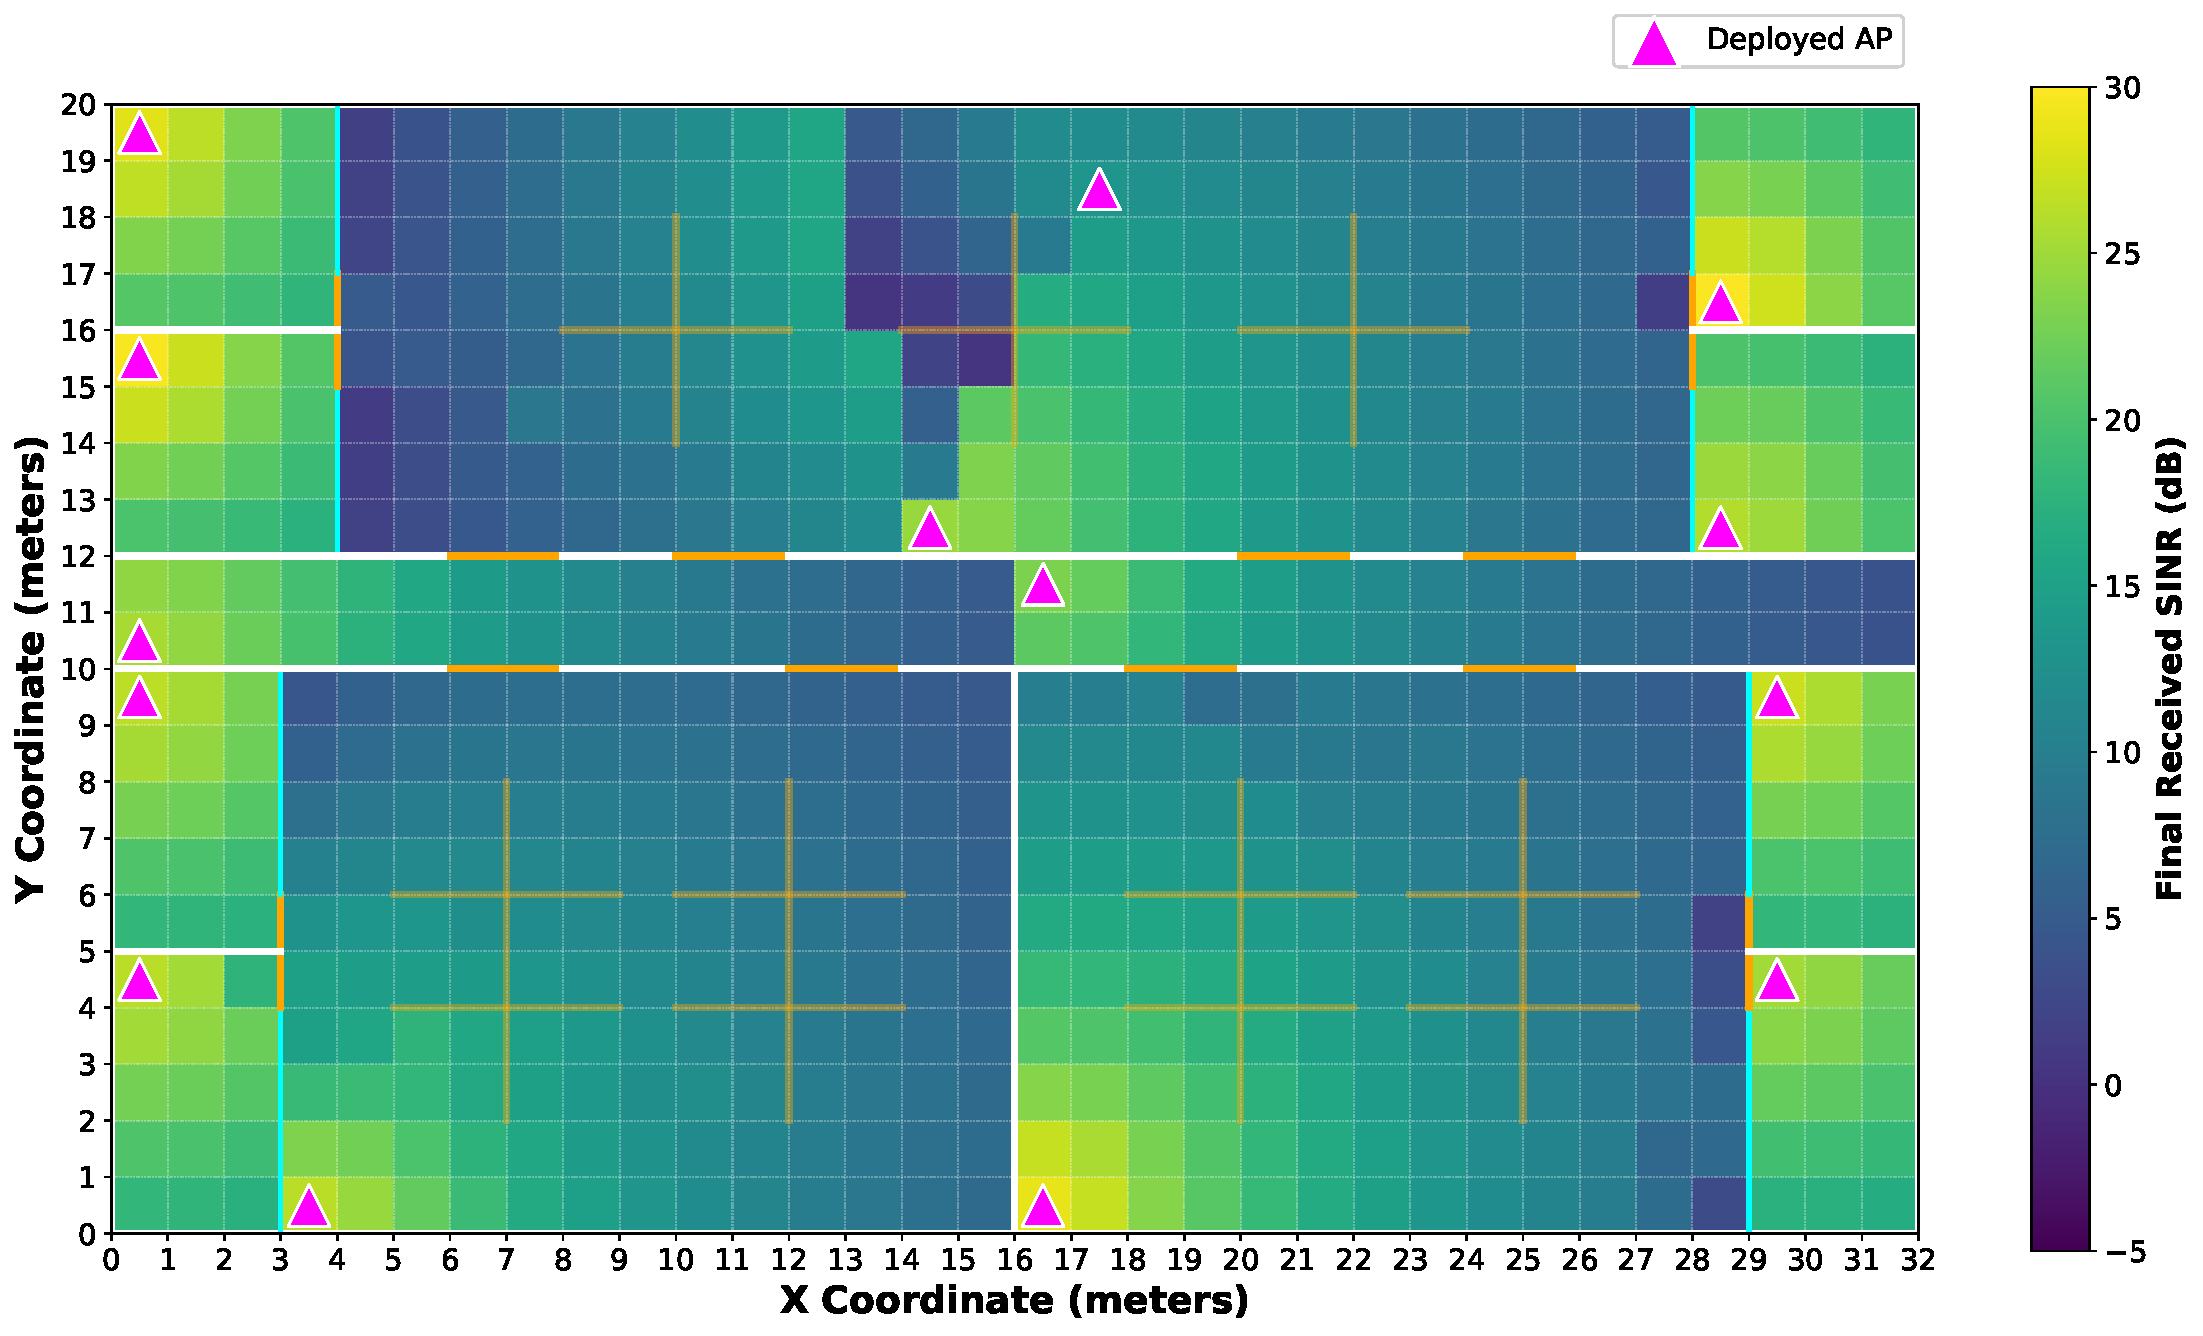
\includegraphics[width=0.95\columnwidth]{thz_sinr_heatmap.pdf}
		\vspace{-8pt}
		\caption{SINR distribution achieving 100\% coverage.}
		\label{fig:static_heatmap}
		\vspace{-10pt}
	\end{figure}
	
	% \subsection{Impact of Dynamic Human Blockages}
	
	% While the static MILP approach produces an optimal layout for an empty room, real environments involve constant human movement. When pedestrian crowds shift into the covered area, the static 14-AP layout experiences severe signal drops, with coverage falling to as low as 16.6\%. This degradation highlights the sensitivity of static THz infrastructure to crowd density.
	
	% To evaluate this, we use a normalized human density score $D_h(c)$ for each grid cell, representing the local footfall relative to the maximum footfall in the area. We define a density threshold ($\tau$) so that cells with $D_h(c) \ge \tau$ are treated as critical zones that must meet the $5$~dB SINR requirement. Adjusting $\tau$ controls the balance between infrastructure cost and coverage guarantees. A stringent threshold (e.g., $\tau = 0.001$) demands near-ubiquitous coverage, which would necessitate 26 APs. Raising $\tau$ to $0.100$ lowers the requirement to 15 APs (covering 60\% of the total area), and setting it to $0.200$ requires only 3 APs (covering 41.3\% of the area). The rapid increase in required APs at lower thresholds indicates that statically deploying hardware to cover all potential crowd layouts is cost-prohibitive. This motivates the need for dynamic AP repositioning to efficiently maintain reliable coverage.
	
	\subsection{Tier-wise Coverage and Displacement Analysis}
	
	We tested the 4-tier cascading HPSO under human blockage conditions that drop initial coverage to 63.6\% (a moderate blockage scenario, distinct from the severe 16.6\% drop evaluated in Section V-C). Table~\ref{tab:tier_summary} summarizes each tier's contribution. From a 14-AP baseline, Tier~2 recovers 26.5~pp (to 90.1\%) without any physical movement ($0.0$~m). Tier~3 adds 3.5~pp for just $3.1$~m of displacement, and Tier~4 contributes a final 3.3~pp at $10.7$~m, restoring total coverage to 96.9\%.

	Importantly, our evaluation assumes ideal, zero-cost user re-association to the best available AP. Thus, the reported coverage collapses represent residual outages occurring despite best-server handovers, underscoring the absolute necessity of physical AP reconfiguration.
	
	% \begin{figure}[t]
		% \centering
		% \includegraphics[width=\columnwidth]{fig3_marginal_improvement.png}
		% \caption{Incremental coverage improvement at each optimization tier.}
		% \vspace{-5pt}
		% \label{fig:marginal_improvement}
		% \end{figure}
	%remove the fig 2 
	\begin{table}[htbp]
		\centering
		\caption{Tier-wise Coverage and Displacement Summary}
		\label{tab:tier_summary}
		\resizebox{\columnwidth}{!}{%
			\begin{tabular}{@{} l c c l @{}}
				\toprule
				\textbf{Tier} & \textbf{Coverage Gain (pp)} & \textbf{Displacement (m)} & \textbf{Adjustment Type} \\
				\midrule
				Baseline & 63.6\% (Initial) & 0.0 & None \\
				Tier~2 & +26.5 & 0.0 & Electronic (beam steering) \\
				Tier~3 & +3.5 & 3.1 & Minor physical (Z-axis) \\
				Tier~4 & +3.3 & 10.7 & Full 3D repositioning \\
				\bottomrule
			\end{tabular}%
		}
		\vspace{-10pt}
	\end{table}
	
	\begin{figure*}[!t]
		\centering
		\begin{minipage}{0.32\textwidth}
			\centering
			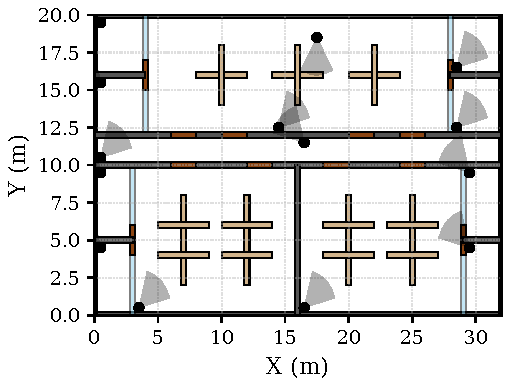
\includegraphics[width=0.9\linewidth]{APSO_Results/ap_placement_t1_before.pdf}
			\vspace{2pt}
			\centerline{\small (a) Step 1: Baseline AP Positions}
			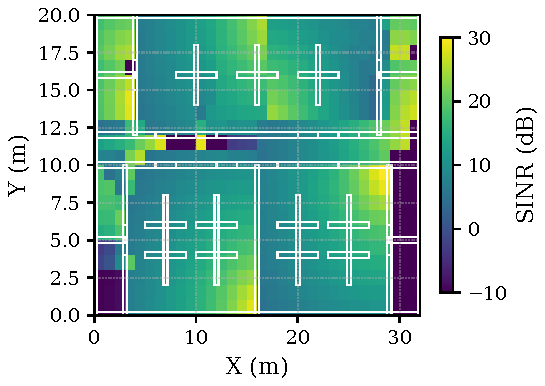
\includegraphics[width=0.9\linewidth]{APSO_Results/sinr_t0_after.pdf}
			\vspace{2pt}
			\centerline{\small (b) Step 2: Established Stable SINR}
		\end{minipage}\hfill
		\begin{minipage}{0.32\textwidth}
			\centering
			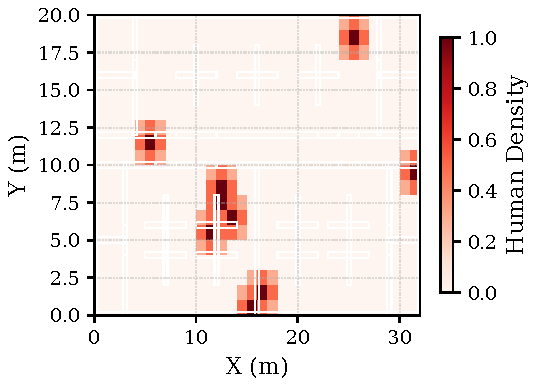
\includegraphics[width=0.9\linewidth]{APSO_Results/density_t1.pdf}
			\vspace{2pt}
			\centerline{\small (c) Step 3: New Human Density Shifts}
			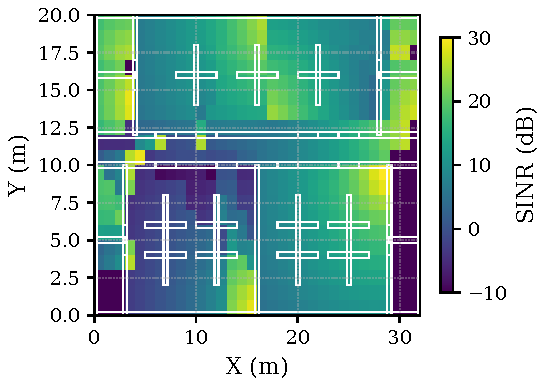
\includegraphics[width=0.9\linewidth]{APSO_Results/sinr_t1_before.pdf}
			\centerline{\small (d) Step 4: Blockage Degrades SINR}
		\end{minipage}\hfill
		\begin{minipage}{0.32\textwidth}
			\centering
			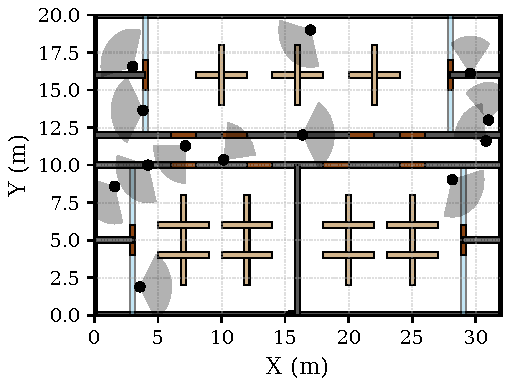
\includegraphics[width=0.9\linewidth]{APSO_Results/ap_placement_t1_after.pdf}
			\centerline{\small (e) Step 5: HPSO Repositions APs}
			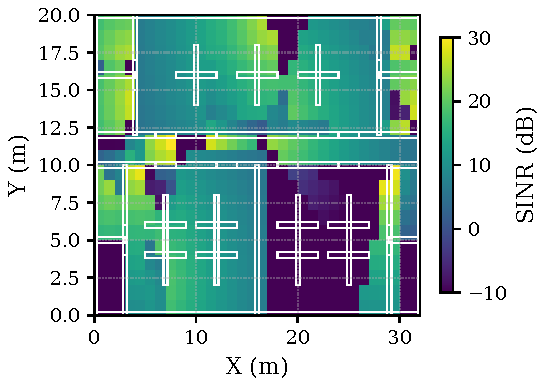
\includegraphics[width=0.9\linewidth]{APSO_Results/sinr_t1_after.pdf}
			\centerline{\small (f) Step 6: Restored SINR Coverage}
		\end{minipage}
		\caption{Adaptation sequence at $t_1$: The $t_0$-optimized AP layout~(a)
			yields stable SINR~(b). A crowd shift~(c) degrades signals~(d), triggering 
			HPSO to reposition and re-angle APs~(e) to restore coverage~(f).}  
		\label{fig:dynamic_lifecycle_combined}
		\vspace{-12pt}
	\end{figure*}
	
	
	The 4-tier approach prioritizes the least disruptive adjustments. Tier~1 retains the existing configuration when coverage is sufficient, conserving computational and mechanical resources. Tier~2 executes the majority of recovery-79\% of the total improvement at zero physical cost by electronically adjusting beam direction and width via phased-array controls in ms, making it highly suitable for real-time mitigation.
	
	Tier~3 is preferred over Tier~4 as minor vertical adjustments consume significantly less time and energy than horizontal robotic relocation. Tier~4 is reserved for when blockage severity renders current AP coordinates entirely unviable. For physical movements in Tiers~3 and~4, the Hungarian assignment algorithm (Section~IV-C2) replaces the nearest-neighbor approach, reducing total movement distance by 8.6\% and saving approximately 4.1~m of travel during the $t_0$ cycle.
	
	\subsection{Temporal Crowd Adaptation}
	
	To evaluate robustness under realistic temporal conditions, we simulated three consecutive crowd shifts at discrete time steps ($t_0, t_1, t_2$), each drawn from an empirical pedestrian mathematical model. At $t_0$, dense crowd clustering drops coverage to 16.6\%; at $t_1$, the crowd redistributes with less severe blockage, yielding 80.2\% initial coverage; at $t_2$, a new dense gathering pattern drops coverage to 58.4\%.
	
	Table~\ref{tab:displacement_over_time} shows the required AP displacement at each timestamp. HPSO recovers coverage from 16.6\% to 97.1\% at $t_0$, from 80.2\% to 95.6\% at $t_1$, and substantially restores coverage from the 58.4\% drop at $t_2$. The $t_1$ adjustment requires only minimal physical displacement, whereas $t_0$ and $t_2$ demand more substantial relocation, highlighting that for less severe crowd shifts, Tier~2 beam steering accounts for most of the recovery with minimal physical movement.
	
	\begin{table}[t]
		\centering
		\caption{AP Mechanical Displacement per Time Step}
		\label{tab:displacement_over_time}
		\begin{tabular}{@{} l c @{}}
			\toprule
			\textbf{Time Step} & \textbf{Total Displacement (m)} \\
			\midrule
			$t_0$ & 42.6 \\
			$t_1$ & 3.0 \\
			$t_2$ & 23.5 \\
			\bottomrule
		\end{tabular}
		\vspace{-10pt}
	\end{table}
	
	Fig.~\ref{fig:dynamic_lifecycle_combined} presents the adaptation sequence at $t_1$: from the $t_0$-optimized AP configuration~(a) and stable SINR~(b), a new crowd shift~(c) degrades coverage~(d), and HPSO repositions and re-angles APs~(e) to fully restore SINR~(f), illustrating the framework's real-time response to dynamic blockages.
	
	
	
	
	\subsection{Comparison with Alternative Approaches}
	
	We evaluate HPSO against standard Particle Swarm Optimization (PSO) and a Genetic Algorithm (GA). Combinatorial approaches such as Greedy Set Cover are excluded because they discard MILP-derived AP positional states, treating each time step independently and failing to preserve the physical movement continuity required for router swarms. The unconstrained PSO serves as a baseline to isolate the benefits of hierarchical tier constraints; it optimizes the identical composite objective function Eq.~(19) (including displacement penalty $\beta M$) but without tier-clamping, updating all 3D coordinates and beam parameters simultaneously. GA serves as a population-based benchmark to verify improvements are not PSO-specific. Simulations use swarm size $S = 50$, maximum iterations $T = 20$, evaluated over 30 Monte Carlo runs with independent random seeds.
	
	Fig.~\ref{fig:coverage_vs_density} illustrates network coverage as human density increases. By incorporating footfall density into the fitness function, HPSO maintains over 88\% coverage under dense blockage scenarios, whereas standard PSO degrades to approximately 74\%. 
	
	The hierarchical structure reduces mechanical movement by prioritizing electronic beam-steering before physical relocation. Standard PSO incurs total displacement exceeding 450~m across the simulated scenarios, whereas the hierarchical model limits displacement to 69.1~m—a 84.6\% reduction. During a severe single blockage event, HPSO requires significantly less displacement (42.6~m) than the 205.8~m of standard PSO, while maintaining high coverage.
	
	\begin{figure}[t]
		\centering
		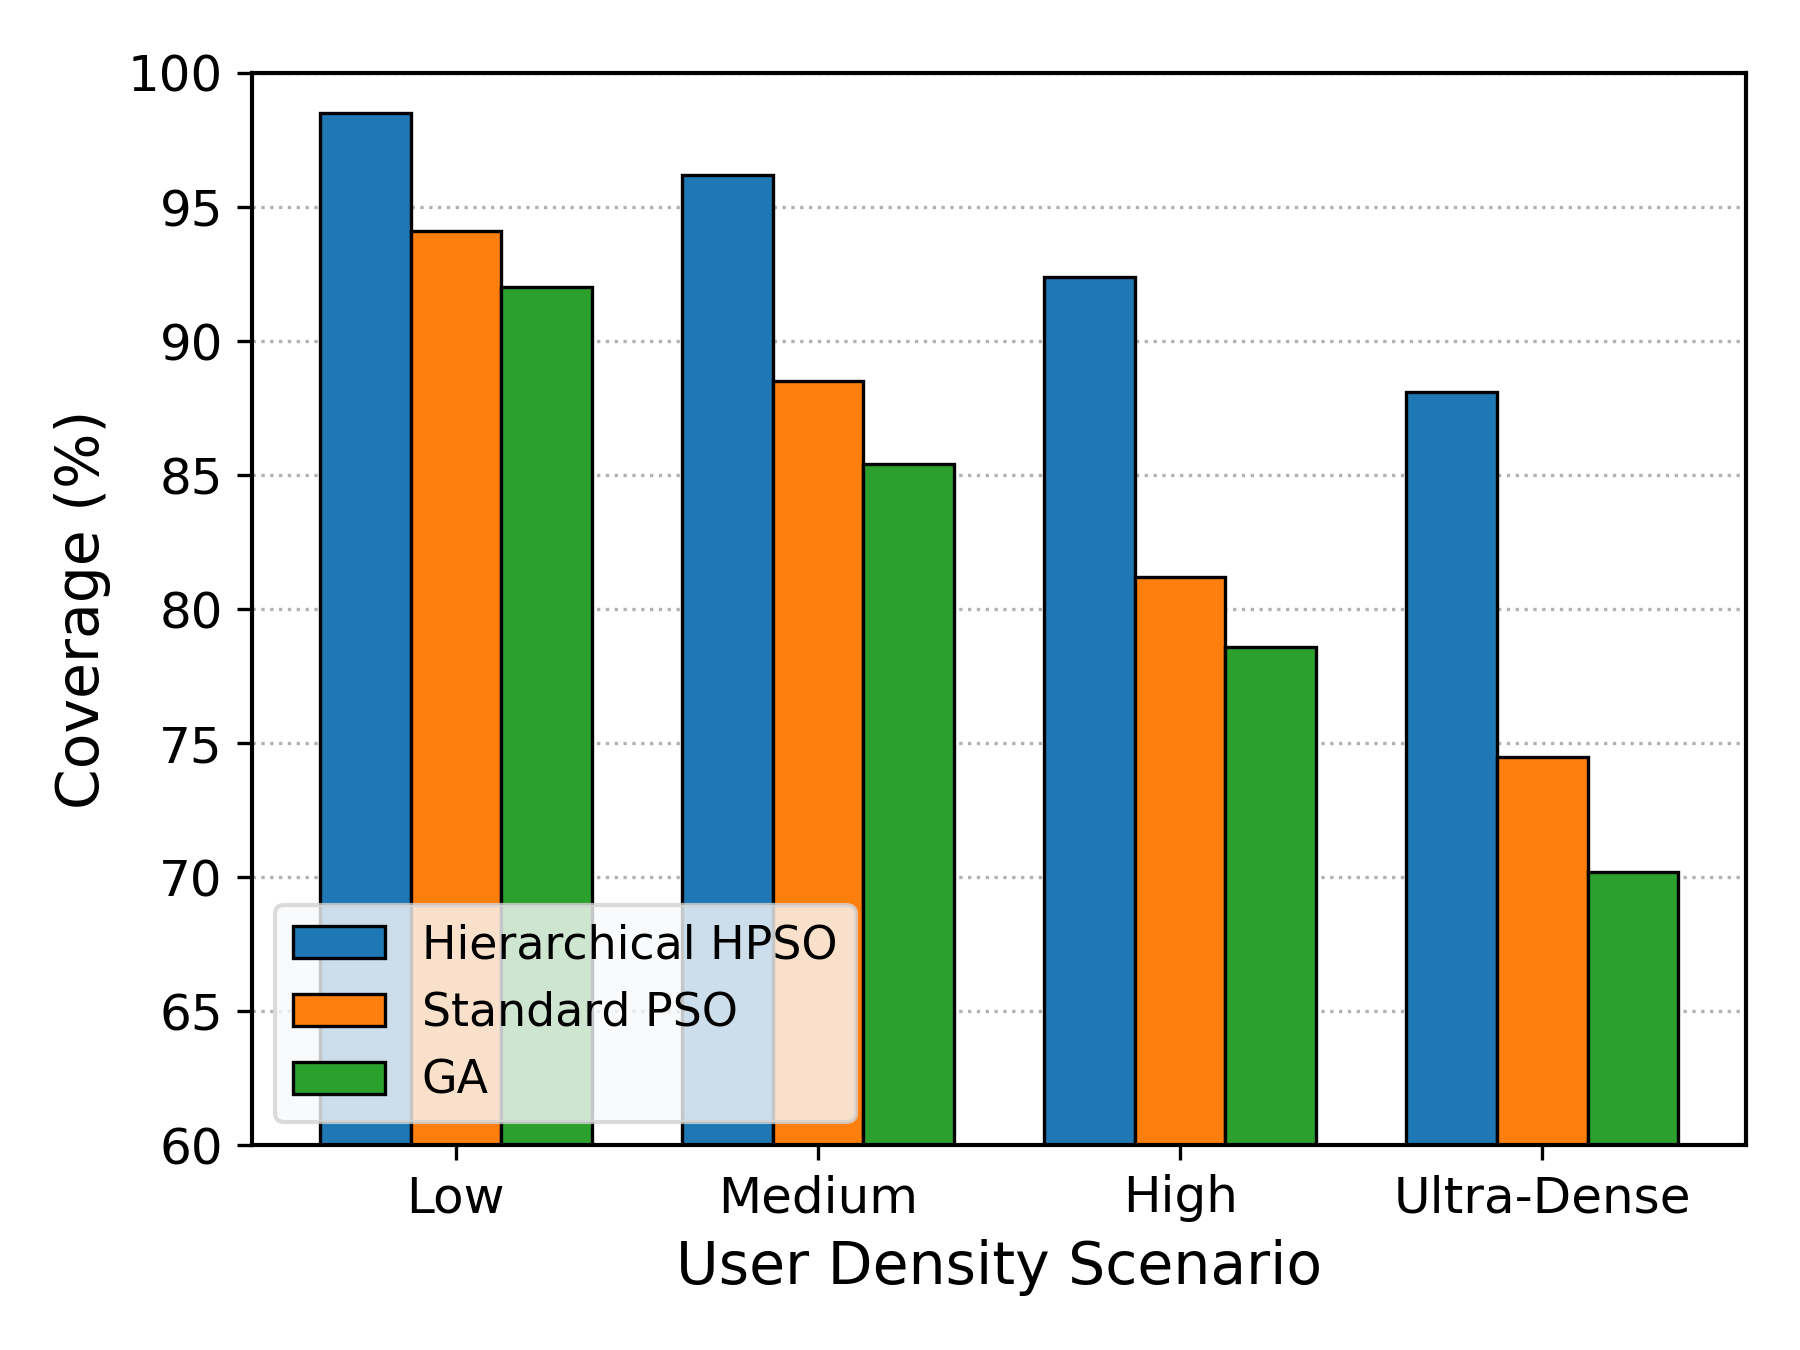
\includegraphics[width=0.80\columnwidth]{fig2_coverage_vs_density.png}
		\caption{Comparison of HPSO with Standard PSO and Genetic Algorithm}
		\vspace{-8pt}
		\label{fig:coverage_vs_density}
	\end{figure}
	
	
	\section{Discussion}
	
	The results presented in this work demonstrate the efficacy of the 4-tier cascading HPSO framework, but the practical deployment of this system can be realized through two distinct operational paradigms: real-time reactive adaptation or scheduled time-based adaptation.
	
	% In a \textbf{real-time adaptation model}, the HPSO framework uses real-time crowd sensing mechanisms to continuously generate the human density spatial matrix. Whenever coverage falls below the 90\% threshold, HPSO is triggered. By relying on Tier 2 electronic beam steering, the framework corrects blockages without physical movement, while Tiers 3 and 4 are activated only when beam steering is insufficient.
	
	% Alternatively, the framework can be deployed as a \textbf{time-based scheduled system}. Human mobility in large indoor environments such as universities or corporate offices may follow recurring temporal patterns. Historical footfall data can be used to predict density patterns at specific times and pre-compute the optimal AP configurations. At the scheduled time, the APs execute the required beam steering and, when necessary, physical repositioning to match the pre-computed configuration, enabling predictive coverage without continuous environmental sensing.
	
	% From a \textbf{mechanical infrastructure} perspective, Tiers 3 and 4 require motorised mounting systems for physical AP movement. Tier 3 can use linear actuators for height adjustment, while Tier 4 can use the ceiling-mounted robotic rails for full 3D repositioning. Flexible PoE cable management can maintain connectivity during the movement. The Hungarian algorithm minimizes the total AP displacement during each cycle.
	
	
	In a \textbf{real-time adaptation model}, HPSO continuously updates the human-density spatial matrix using crowd-sensing data such as LiDAR, and is activated when coverage falls below 90\%. Tier 2 first handles the blockage using electronic beam steering. If this is not enough, Tiers 3 and 4 adjust the AP height and perform full 3D repositioning. Alternatively, a \textbf{time-based scheduled system} can use historical footfall data to estimate density patterns and pre-compute AP configurations for specific times, avoiding the need for continuous sensing. For physical movement, Tier 3 can use linear actuators, while Tier 4 can use ceiling-mounted robotic rails. Flexible PoE cable management keeps the APs connected during movement. The Hungarian algorithm is used to minimize the total AP displacement during each reconfiguration cycle.

	Finally, while this framework demonstrates the theoretical gains of mobility, practical deployments must account for actuation latency (e.g., rails moving at $0.2$~m/s take seconds to relocate APs) and the upfront hardware cost of robotic infrastructure compared to denser static over-provisioning.
	
	
	\section{Conclusion}
	
	This paper presents a comprehensive framework for 6G Terahertz (THz) Access Point deployment, bridging the gap between theoretical limits and unpredictable indoor environments. We initially demonstrated that optimizing AP height and beam orientation via a 3D MILP formulation significantly reduces the required number of APs. However, because static models inevitably degrade when moving human crowds block fragile high-frequency signals, we introduced a human density metric to continuously track spatial blockage. 
	
	To overcome these blockages, we developed a 4-tier Hierarchical Particle Swarm Optimization (HPSO) architecture. By hierarchically escalating from fast, zero-movement electronic beam steering up to full 3D robotic repositioning only when absolutely necessary, our framework successfully restores network coverage even during dense crowd shifts. Reinforced by the Hungarian algorithm to minimize mechanical displacement, this research demonstrates that reliable THz networks can be achieved by intelligently and dynamically adapting to the crowds they serve, rather than statically over-provisioning APs.
	
	\begin{thebibliography}{00}
		\bibitem{b1} T. S. Rappaport et al., ``Millimeter Wave Mobile Communications for 5G Cellular: It Will Work!,'' \textit{IEEE Access}, vol. 1, pp. 335-349, 2013.
		
		\bibitem{b2} Y. Niu et al., ``A survey of millimeter wave communications (mmWave) for 5G: opportunities and challenges,\'\' \textit{Wireless Networks}, vol. 21, pp. 2657-2676, 2015.

	\bibitem{b4}
	A. M. Baswade, S. Kiran M. R., B. R. Tamma, and A. Franklin,
	``On Placement of LAA/LTE-U Base Stations in Heterogeneous Wireless Networks,\'\' in \textit{Proc. 19th Int. Conf. Distributed Computing and Networking (ICDCN)}, 2018, pp. 37:1--37:10.
		
		
		
		\bibitem{b5} I. F. Akyildiz, J. M. Jornet, and C. Han, ``Terahertz band: Next frontier for wireless communications,'' \textit{Physical Communication}, vol. 12, pp. 16--32, 2014.
		
		\bibitem{b6}
		B. A. Bilgin, H. Ramezani, and O. B. Akan,
		``Human Blockage Model for Indoor Terahertz Band Communication,''
		in \textit{Proc. IEEE Int. Conf. Commun. Workshops (ICC Workshops)},
		2019, pp. 1--6, doi: 10.1109/ICCW.2019.8757158.
		
		\bibitem{b7}
		Y. Liu, Y. Jian, R. Sivakumar, and D. M. Blough,
		``Maximizing Line-of-Sight Coverage for mmWave Wireless LANs With
		Multiple Access Points,'' \textit{IEEE/ACM Trans. Netw.}, vol. 30,
		no. 2, pp. 698--716, 2022, doi: 10.1109/TNET.2021.3122378.
		
		
		
		\bibitem{b11} J. Kennedy and R. Eberhart, ``Particle swarm optimization,'' in \textit{Proc. IEEE Int. Conf. Neural Networks (ICNN)}, Perth, Australia, 1995, vol. 4, pp. 1942--1948.
		
		\bibitem{b12} H. W. Kuhn, ``The Hungarian method for the assignment problem,'' \textit{Naval Research Logistics Quarterly}, vol. 2, no. 1--2, pp. 83--97, 1955.
		
		\bibitem{b13} Y. Shi and R. Eberhart, ``A modified particle swarm optimizer,'' in \textit{Proc. IEEE Int. Conf. Evolutionary Computation (ICEC)}, Anchorage, AK, USA, 1998, pp. 69--73.
		
		\bibitem{b14}
		V. Petrov, M. Komarov, D. Moltchanov, J. M. Jornet, and
		Y. Koucheryavy, ``Interference and SINR in Millimeter Wave and
		Terahertz Communication Systems With Blocking and Directional
		Antennas,'' \textit{IEEE Trans. Wireless Commun.}, vol.~16, no.~3,
		pp.~1791--1808, 2017, doi: 10.1109/TWC.2017.2654351.
		
		\bibitem{b15}
		M. Alzenad, A. El-Keyi, F. Lagum, and H. Yanikomeroglu,
		``3-D Placement of an Unmanned Aerial Vehicle Base Station (UAV-BS)
		for Energy-Efficient Maximal Coverage,'' \textit{IEEE Wireless
			Commun. Lett.}, vol.~6, no.~4, pp.~434--437, 2017,
		doi: 10.1109/LWC.2017.2700840.
		
		\bibitem{b16}
		T. A. Kareem, M. A. Hussain, and M. K. Jabbar,
		``Particle Swarm Optimization Based Beamforming in Massive MIMO
		Systems,'' \textit{Int. J. Interact. Mob. Technol.}, vol.~14,
		no.~5, pp.~176--192, 2020,
		doi: 10.3991/IJIM.V14I05.13701.
		
		\bibitem{b20}
		Y. Zhou \textit{et al.}, ``Terahertz Meets Untrusted UAV-Relaying:
		Minimum Secrecy Energy Efficiency Maximization via Trajectory and
		Communication Co-Design,'' \textit{IEEE Trans. Veh. Technol.},
		vol.~71, no.~5, pp.~4991--5006, 2022,
		doi: 10.1109/TVT.2022.3150011.
		
		\bibitem{b21}
		T. Murakami, S. Oka, Y. Takatori, M. Mizoguchi, and F. Maehara,
		``On the Feasibility of an Adaptive Movable Access Point System in a
		Static Indoor WLAN Environment,'' \textit{IEICE Trans. Commun.},
		vol.~E101-B, no.~7, pp.~1693--1700, 2018,
		doi: 10.1587/transcom.2017EBP3291.
		
		\bibitem{b22}
		L. Zhu, W. Ma, and R. Zhang, ``Movable Antennas for Wireless
		Communication: Opportunities and Challenges,'' \textit{IEEE Commun.
			Mag.}, vol.~62, no.~6, pp.~114--120, 2024,
		doi: 10.1109/MCOM.001.2300212.
		
		\bibitem{b25}
		G. Charan, M. Alrabeiah, and A. Alkhateeb, ``Vision-Aided 6G
		Wireless Communications: Blockage Prediction and Proactive Handoff,''
		\textit{IEEE Trans. Veh. Technol.}, vol.~70, no.~10,
		pp.~10193--10208, 2021,
		doi: 10.1109/TVT.2021.3104219.
		\bibitem{b27}
		S. Kim \textit{et al.}, ``Human Recognition and Tracking in Narrow Indoor Environment using 3D Lidar Sensor,'' in \textit{2020 20th International Conference on Control, Automation and Systems (ICCAS)}, 2020, pp. 1--4, doi: 10.23919/ICCAS50221.2020.9268208.
		
		\bibitem{b29}
		T. Linder \textit{et al.}, ``InLiDa: A 3D Lidar Dataset for People Detection and Tracking in Indoor Environments,'' in \textit{Proc. 12th Int. Joint Conf. Comput. Vis., Imaging and Comput. Graph. Theory and Appl. (VISAPP)}, 2017, pp. 433--440, doi: 10.5220/0006148704840491.
		
		
	\end{thebibliography}
	
\end{document}
